%% LaTeX-Beamer template for KIT design
%% by Erik Burger, Christian Hammer
%% title picture by Klaus Krogmann
%%
%% version 2.1
%%
%% mostly compatible to KIT corporate design v2.0
%% http://intranet.kit.edu/gestaltungsrichtlinien.php
%%
%% Problems, bugs and comments to
%% burger@kit.edu

\documentclass[19pt]{beamer}

%% SLIDE FORMAT

% use 'beamerthemekit' for standard 4:3 ratio
% for widescreen slides (16:9), use 'beamerthemekitwide'

\usepackage{templates/beamerthemekit}
\usepackage{wrapfig}

\usepackage[utf8]{inputenc}
\usepackage[T1]{fontenc}
\usepackage[ngerman]{babel}	% german hyphenation, quotes, etc
\usepackage{tikz}
\usepackage{hyperref}
% \usepackage[ngerman]{translator}

% \usepackage{templates/beamerthemekitwide}

%% TITLE PICTURE

% if a custom picture is to be used on the title page, copy it into the 'logos'
% directory, in the line below, replace 'mypicture' with the 
% filename (without extension) and uncomment the following line
% (picture proportions: 63 : 20 for standard, 169 : 40 for wide
% *.eps format if you use latex+dvips+ps2pdf, 
% *.jpg/*.png/*.pdf if you use pdflatex)
\titleimage{Gruppenarbeit_klein}

%% TITLE LOGO

% for a custom logo on the front page, copy your file into the 'logos'
% directory, insert the filename in the line below and uncomment it

\titlelogo{Logo_IOSB}

% (*.eps format if you use latex+dvips+ps2pdf,
% *.jpg/*.png/*.pdf if you use pdflatex)

%% TikZ INTEGRATION

% use these packages for PCM symbols and UML classes
% \usepackage{templates/tikzkit}
% \usepackage{templates/tikzuml}

% the presentation starts here

\title[PCC]{Privacy Crash Cam:\\ Entwurf}
\subtitle{App, Web-Interface und Web-Dienst}
\author{Giorgio G., Christoph H., David L.,  Josh R.,  Fabian W.}

\institute{Karlsruher Institut f\"ur Technologie, Fraunhofer Institut f\"ur Optronik, Systemtechnik und Bildauswertung}

% Bibliography

\usepackage[citestyle=authoryear,bibstyle=numeric,hyperref,backend=biber]{biblatex}
\addbibresource{templates/example.bib}
\bibhang1em

\begin{document}

% change the following line to "ngerman" for German style date and logos
\selectlanguage{ngerman}

%title page
\begin{frame}
	\titlepage
\end{frame}

%###############################################################################################

\section{Aufgabenstellung}
\begin{frame}{Aufgabenstellung}
	\begin{itemize}
		\item Funktionsfähiger Entwurf nach Vorgaben des Pflichtenhefts
		\pause
		\item Aussagekräftige Klassendiagramme
		\pause
		\item Beschreibung der Klassen, Module, Datenspeicherung und Architektur
	\end{itemize}
\end{frame}
\subsection{Ziel}
\begin{frame}{Ziel}
\begin{center}
\begin{tikzpicture}
  \node (img1) {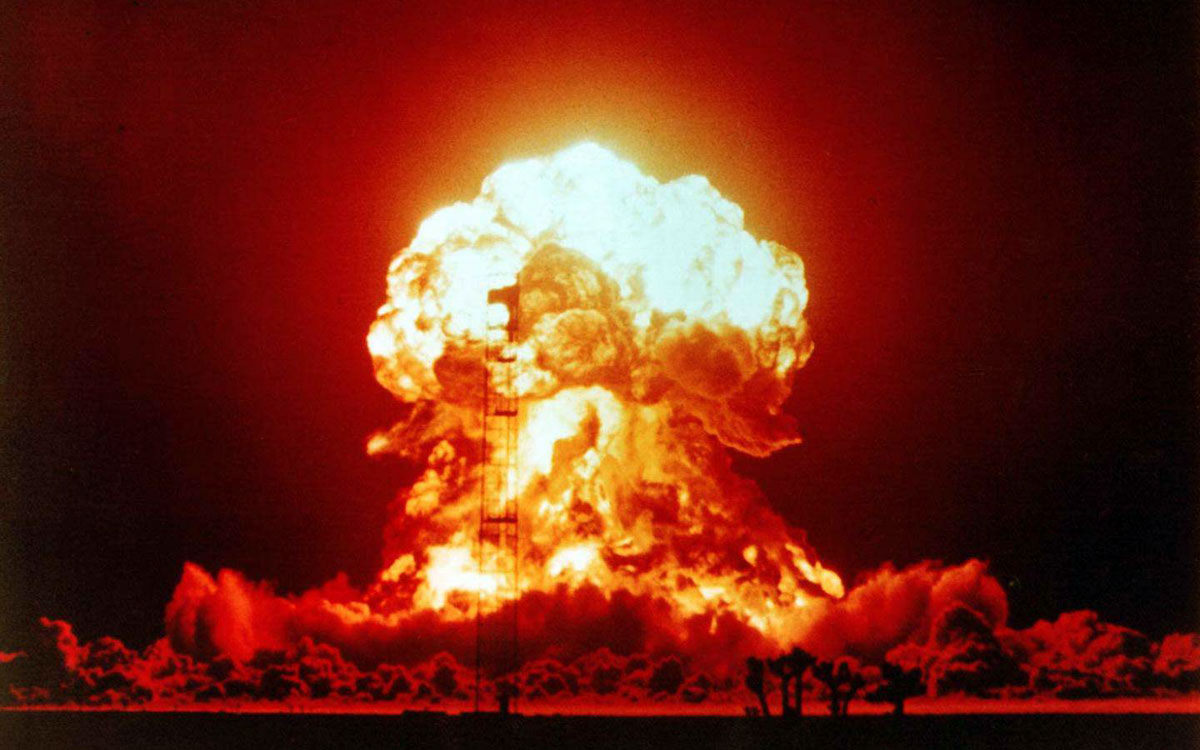
\includegraphics[height=7cm]{resources/explosion.jpg}};
  \node (img2) at (img1.center) {
\includegraphics[height=3cm]{resources/cross.png}};
\end{tikzpicture}
\end{center}
\end{frame}

\section{Vorgehensweise}
\begin{frame}{Vorgehensweise}
\begin{center}
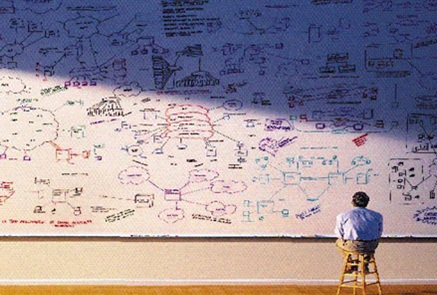
\includegraphics[scale=1]{resources/fing_hard.jpg}
\end{center}
\end{frame}
\subsection{Skizzieren}
\begin{frame}{Skizzieren}
\begin{center}
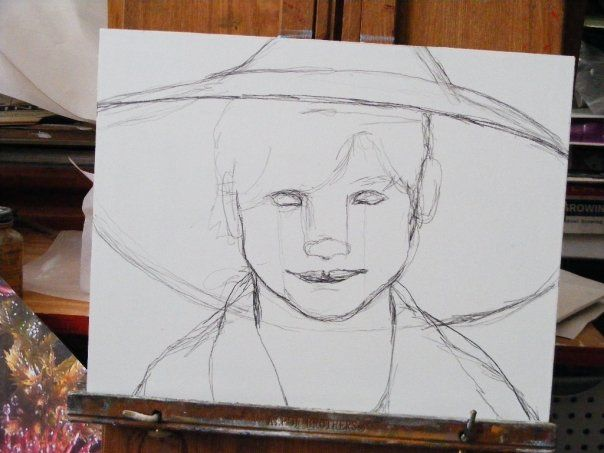
\includegraphics[scale=0.3]{resources/draft.jpg}
\end{center}
\end{frame}
\subsection{Klassenabhängigkeiten + Schnittstellen}
\begin{frame}{Klassenabhängigkeiten + Schnittstellen}
\begin{center}
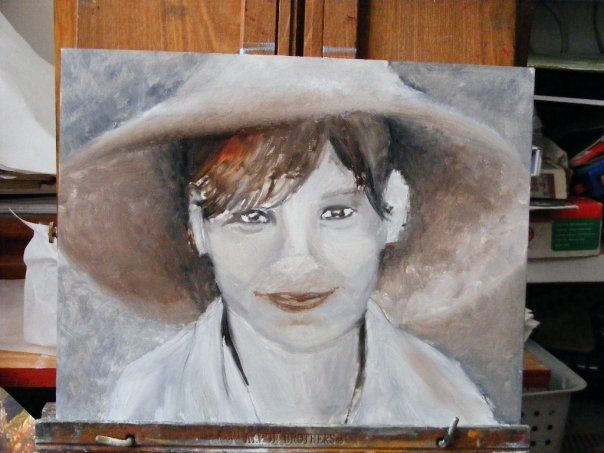
\includegraphics[scale=0.3]{resources/basic_relations.jpg}
\end{center}
\end{frame}
\subsection{Ausarbeitung Klassen + Module}
\begin{frame}{Ausarbeitung Klassen + Module}
\begin{center}

\includegraphics[scale=0.3]{resources/outline.jpg}
\end{center}
\end{frame}
\subsection{Feinschliff}
\begin{frame}{Feinschliff}
\begin{center}
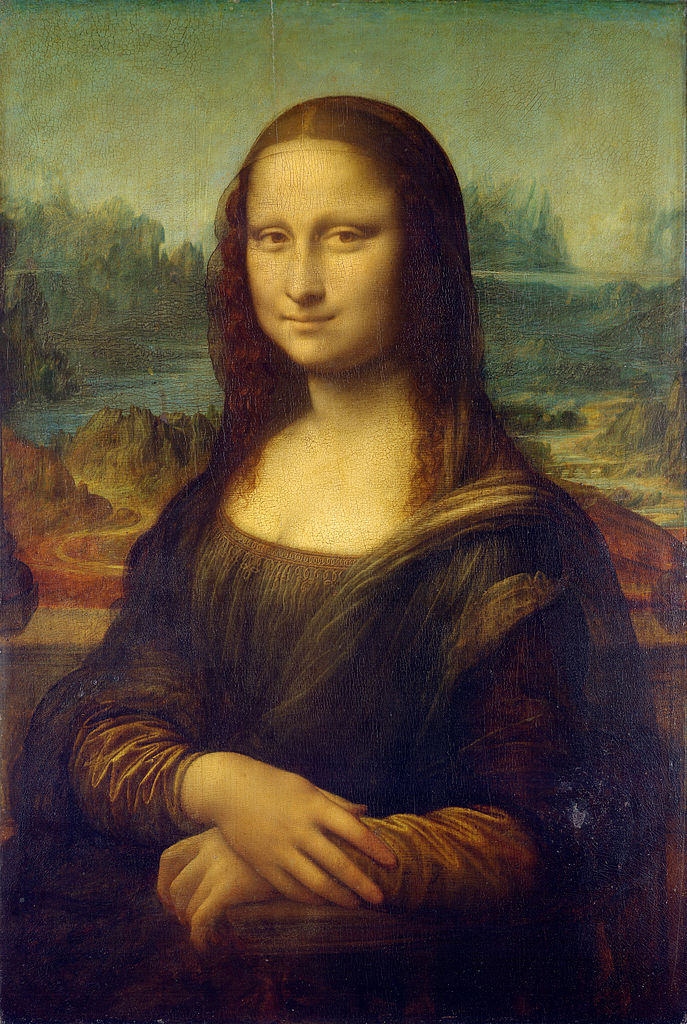
\includegraphics[scale=0.2]{resources/review.jpg}
\end{center}
\end{frame}

% ______________________________ 2 MINUTE MARK

\section{App}
\begin{frame}{App}
	\begin{itemize}
    	\item Vorbereitung
		\begin{itemize}
			\item Vertraut machen mit Android Framework und Designprinzipien
			\pause
			\item Einarbeiten in Camera API und Sensor API
			\pause
		\end{itemize}
		\item Umsetzung Entwurf
		\begin{itemize}
			\item GUI erweiterbar
			\pause
			\item Datenverarbeitung, Netzwerkanfragen, Kamera austauschbar / abgeschottet
			\item -> Entwurfsmuster und -prinzipien angewendet
			\pause
			\item Feinschliff durch bessere Strukturierung und Namensgebung
		\end{itemize}
		\item Besondere Probleme
		\begin{itemize}
			\item Ringpuffer
			\pause
			\item Asynchrone Vorgänge in Android
			\pause 
			\item Kamera-Handling
		\end{itemize}
	\end{itemize}
\end{frame}
\subsection{Ringpuffer}
\begin{frame}{Ringpuffer}
\begin{center}
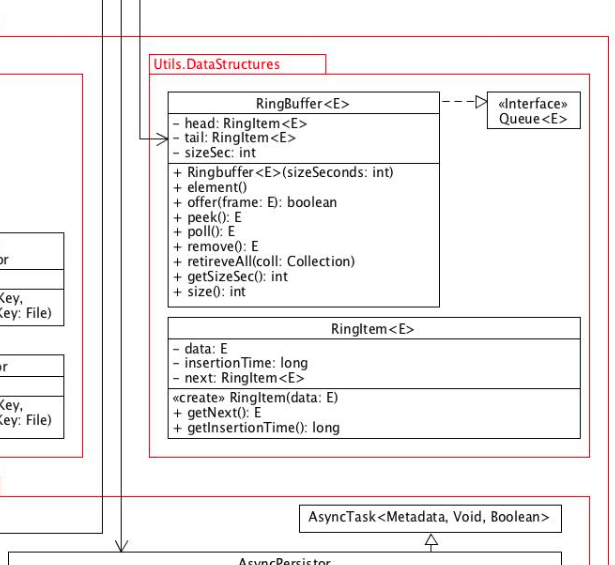
\includegraphics[scale=0.33]{resources/ringbuffer_old.jpg}
\end{center}
\end{frame}
\subsection{Ringpuffer}
\begin{frame}{Ringpuffer}
\begin{center}
% 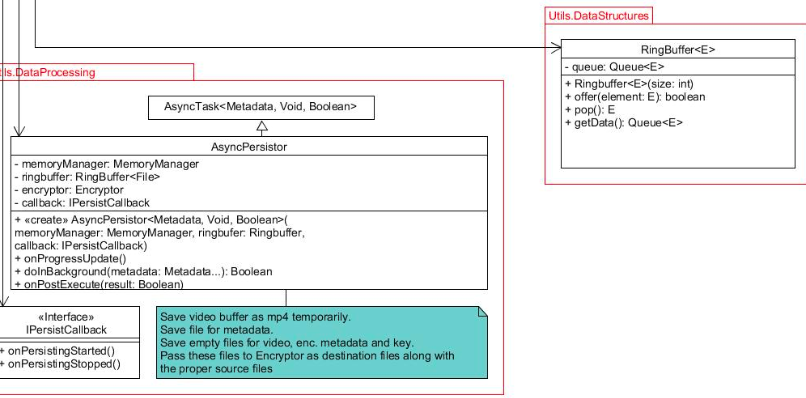
\includegraphics[scale=0.3]{resources/ringbuffer_new.jpg}
\end{center}
\end{frame}

% ______ LEAVE OUT CAMERA (or old new comparison) IF TIME TOO SHORT _______
\subsection{Kamera}
\begin{frame}{Kamera}
\begin{center}
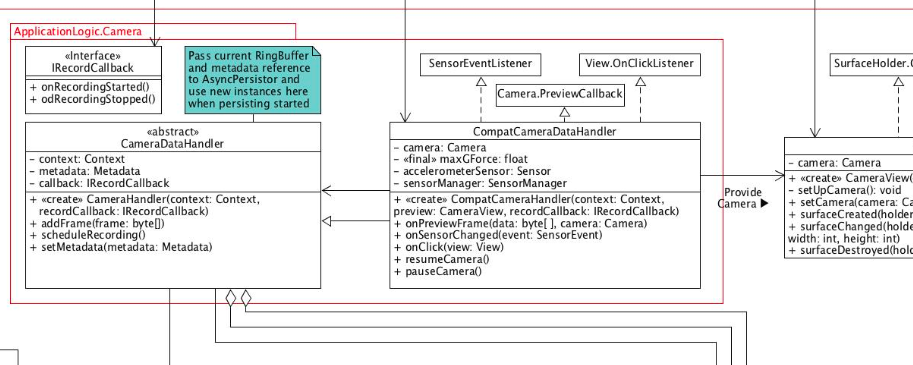
\includegraphics[scale=0.33]{resources/camera_old.jpg}
\end{center}
\end{frame}
\subsection{Kamera}
\begin{frame}{Kamera}
\begin{center}
% 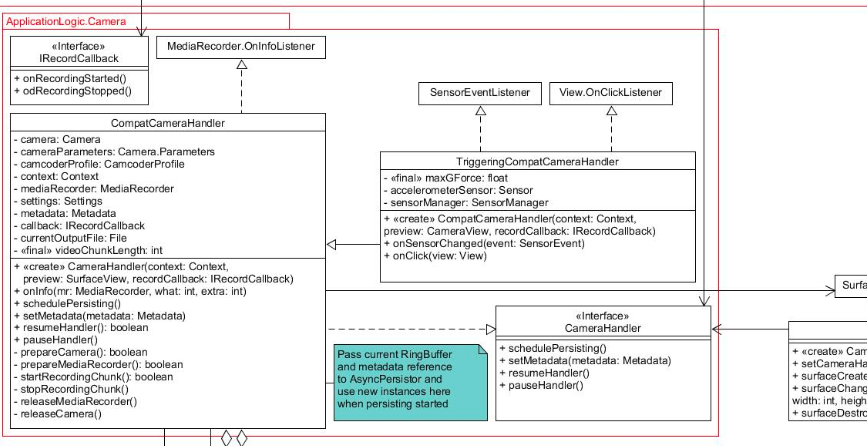
\includegraphics[scale=0.3]{resources/camera_new.jpg}
\end{center}
\end{frame}

% __________________________ 4 MINUTE MARK


\section{Web-Interface}
\begin{frame}{Web-Interface}
    \begin{itemize}
    	\item Vorbereitung
    	\begin{itemize}
			\item Vertraut machen mit Vaadin
			\pause
			\item Analyse von Beispielen und Demos
			\pause
		\end{itemize}
		\item Umsetzung Entwurf
		\begin{itemize}
			\item Entwerfen Grundlegender Struktur einer Gui
			\pause
			\item Anzeige und Logik entkoppeln
			\pause
		\end{itemize}
    	\item Besondere Probleme
    	\begin{itemize}
			\item Entkoppeln von Logik und Anzeige
			\pause
			\item Kommunikation mit dem Web-Dienst
		\end{itemize}
    \end{itemize}
\end{frame}
\subsection{GUI}
\begin{frame}{GUI}
\begin{center}
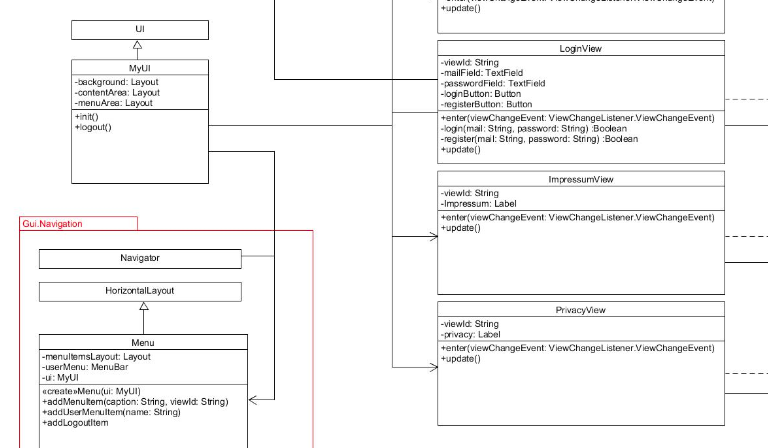
\includegraphics[scale=0.35]{resources/interface_gui.png}
\end{center}
\end{frame}
\subsection{Logik}
\begin{frame}{Logik}
\begin{center}
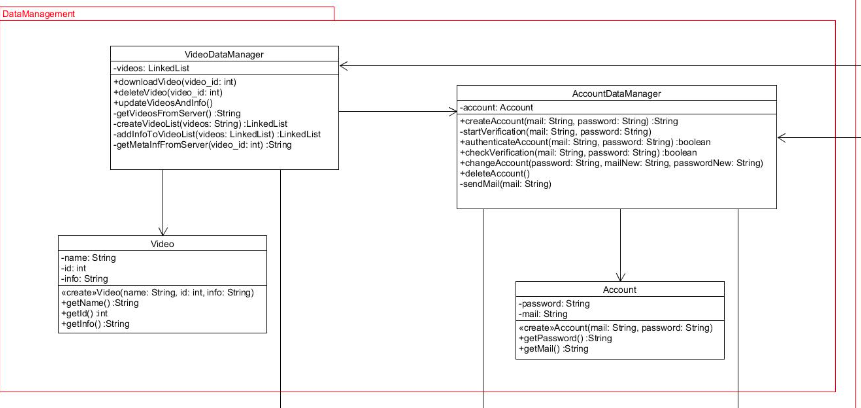
\includegraphics[scale=0.35]{resources/interface_logic.png}
\end{center}
\end{frame}
\subsection{Serveranfragen}
\begin{frame}{Serveranfragen}
\begin{center}
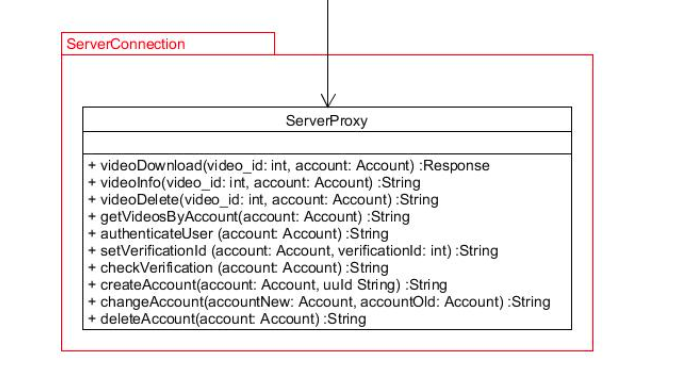
\includegraphics[scale=0.35]{resources/interface_serverconnection.png}
\end{center}
\end{frame}

% __________________________6 MINUTE MARK

\section{Web-Dienst}
\begin{frame}{Web-Dienst}
	\begin{itemize}
		\item Vorbereitung
		\begin{itemize}
			\item Vertraut machen mit Jetty und Jersey
			\pause
			\item Einarbeiten in Rest Anfragen und JSON Objekte
			\pause
		\end{itemize}
		\item Umsetzung Entwurf
		\begin{itemize}
			\item Einheitliche Schnittstelle nach außen
			\pause
			\item Authentifizierung bei jeder Anfrage
			\pause
			\item Schnittstellen, Datenablage und Videoverarbeitung trennen
			\pause
		\end{itemize}
		\item Besondere Probleme
		\begin{itemize}
			\item Videoverarbeitung per Pipeline
			\pause
			\item Großer Umfang an Funktionalität
		\end{itemize}
	\end{itemize}
\end{frame}
\subsection{Schnittstelle}
\begin{frame}{Schnittstelle}
\begin{center}
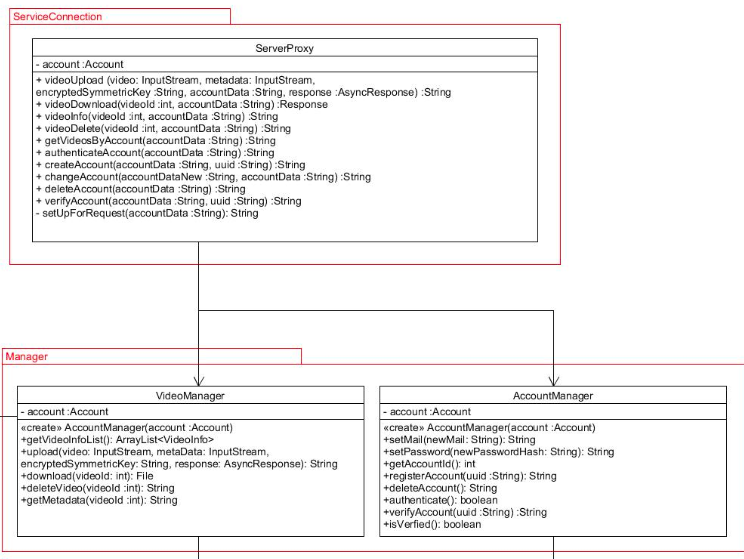
\includegraphics[scale=0.3]{resources/service_rest.png}
\end{center}
\end{frame}
\subsection{Video Chain}
\begin{frame}{Video Chain}
\begin{center}
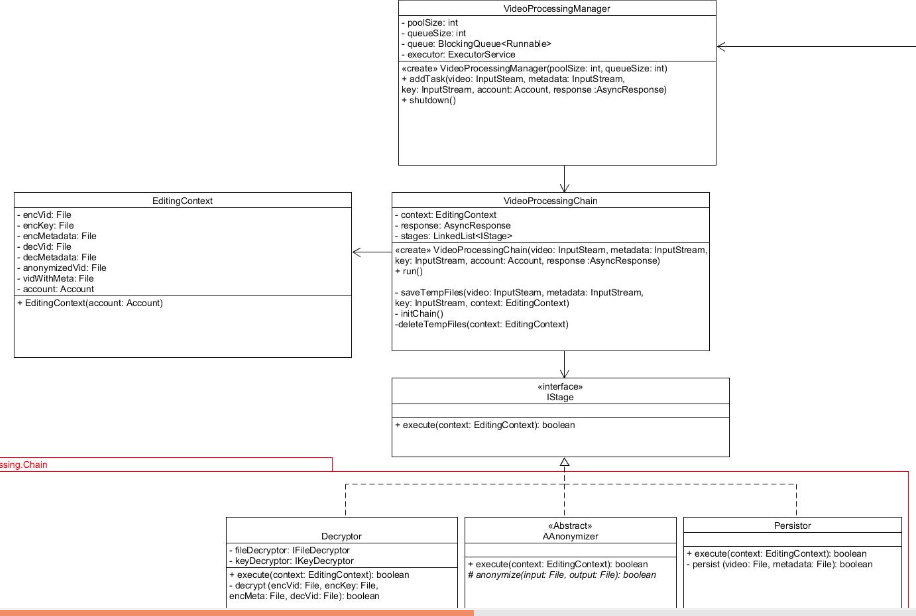
\includegraphics[scale=0.3]{resources/service_vidchain.png}
\end{center}
\end{frame}
\subsection{Datenbank}
\begin{frame}{Datenbank}
\begin{center}
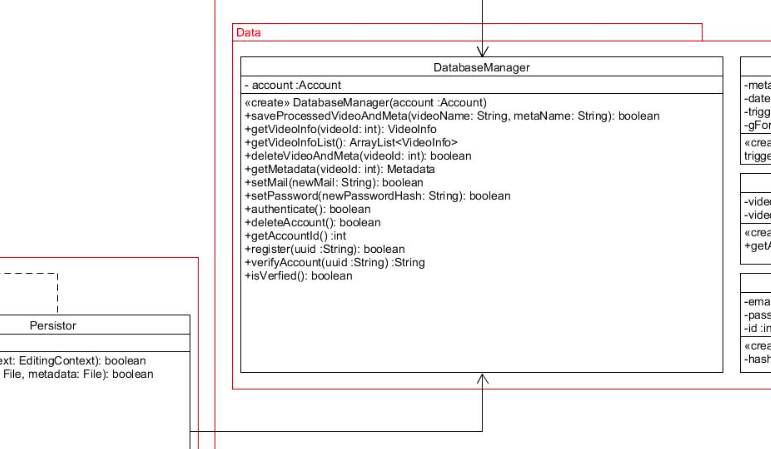
\includegraphics[scale=0.35]{resources/service_db.png}
\end{center}
\end{frame}

% __________________________ 8 MINUTE MARK

\section{Organisation}

\subsection{Aufgabenverteilung}
\begin{frame}{Aufgabenverteilung}
  \begin{columns}[T]
    \begin{column}{.5\textwidth}
    		\begin{itemize}
    	\item Christoph H.
			\begin{itemize}
				\item Web-Interface
				\item Präsentation
			\end{itemize}
		\item David L.
			\begin{itemize}
				\item Web-Dienst
			\end{itemize}
		\item Fabian W.
			\begin{itemize}
				\item Web-Dienst
			\end{itemize}
    		\end{itemize}
    \end{column}
    \begin{column}{.5\textwidth}
    \begin{itemize}
		\item Giorgio G.
			\begin{itemize}
				\item App
				\item Präsentation
			\end{itemize}
		\item Josh R.
			\begin{itemize}
				\item App
				\item Web-Dienst
			\end{itemize}
	\end{itemize}
    \end{column}
  \end{columns}
\end{frame}

\subsection{JIRA}
\begin{frame}{JIRA}
	\begin{figure}
		\begin{center}
			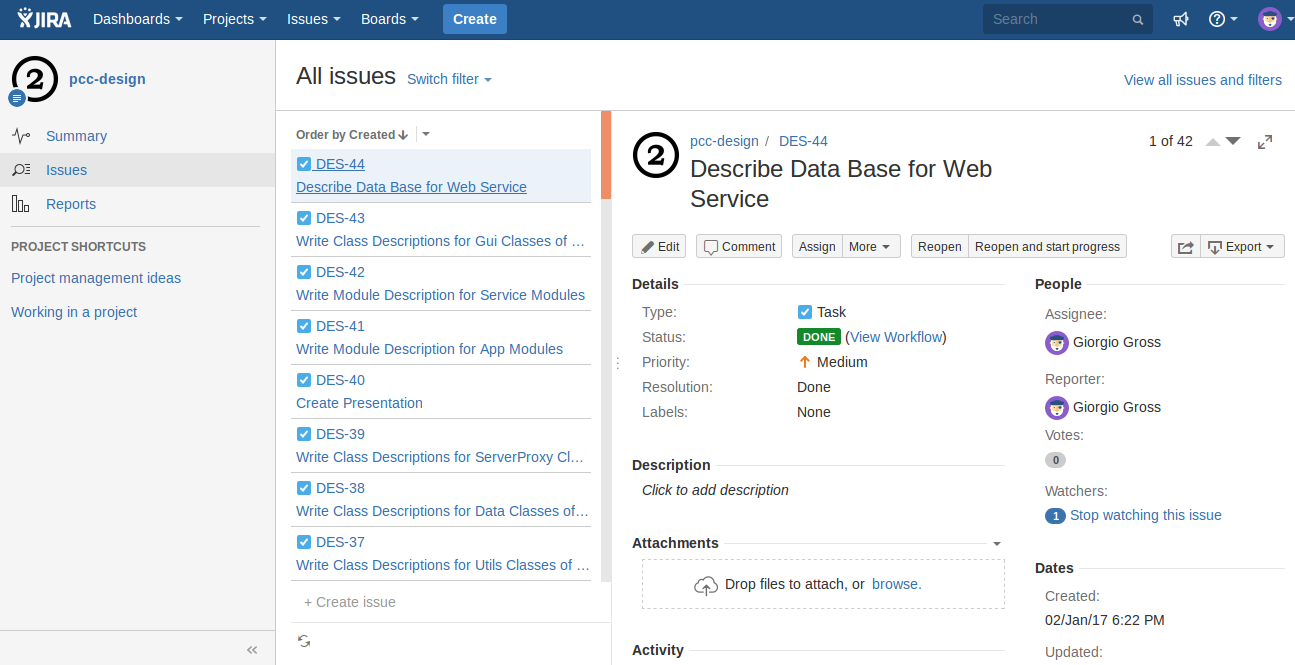
\includegraphics[scale=0.25]{resources/jira_1.jpg} 
		\end{center}
	\end{figure}				
\end{frame}

\subsection{Github}
\begin{frame}{Github} % [allowframebreaks]
	\begin{figure}
		\begin{center}
			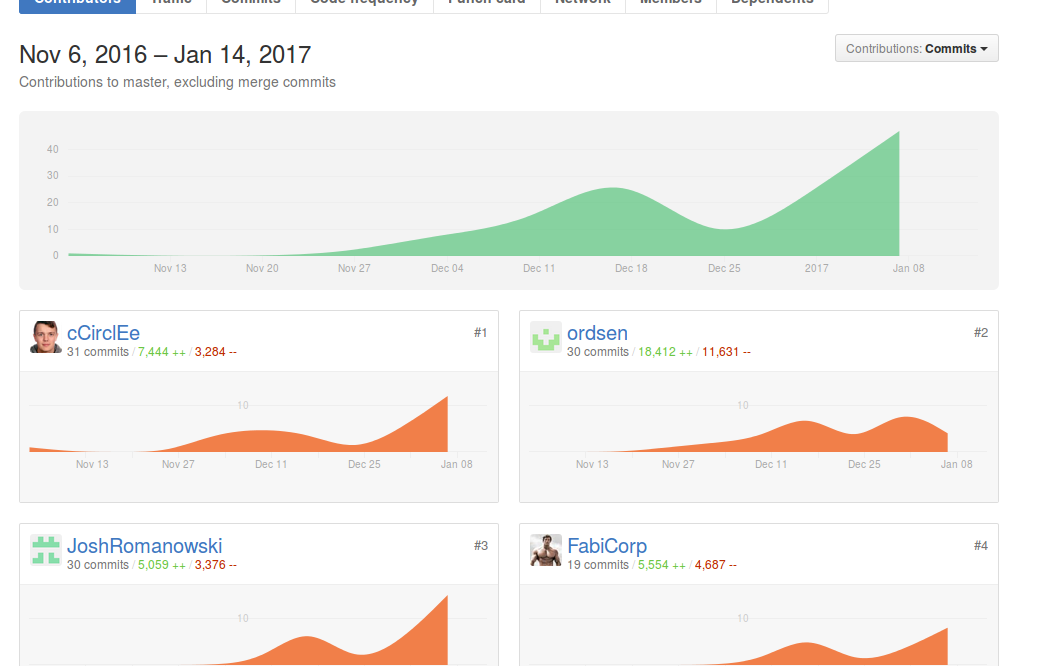
\includegraphics[scale=0.27]{resources/github_stats_commits.png}
		\end{center}
	\end{figure}				
\end{frame}

\section{Gruppenarbeit}
\begin{frame}{Gruppenarbeit}
	\begin{figure}
		\begin{center}
			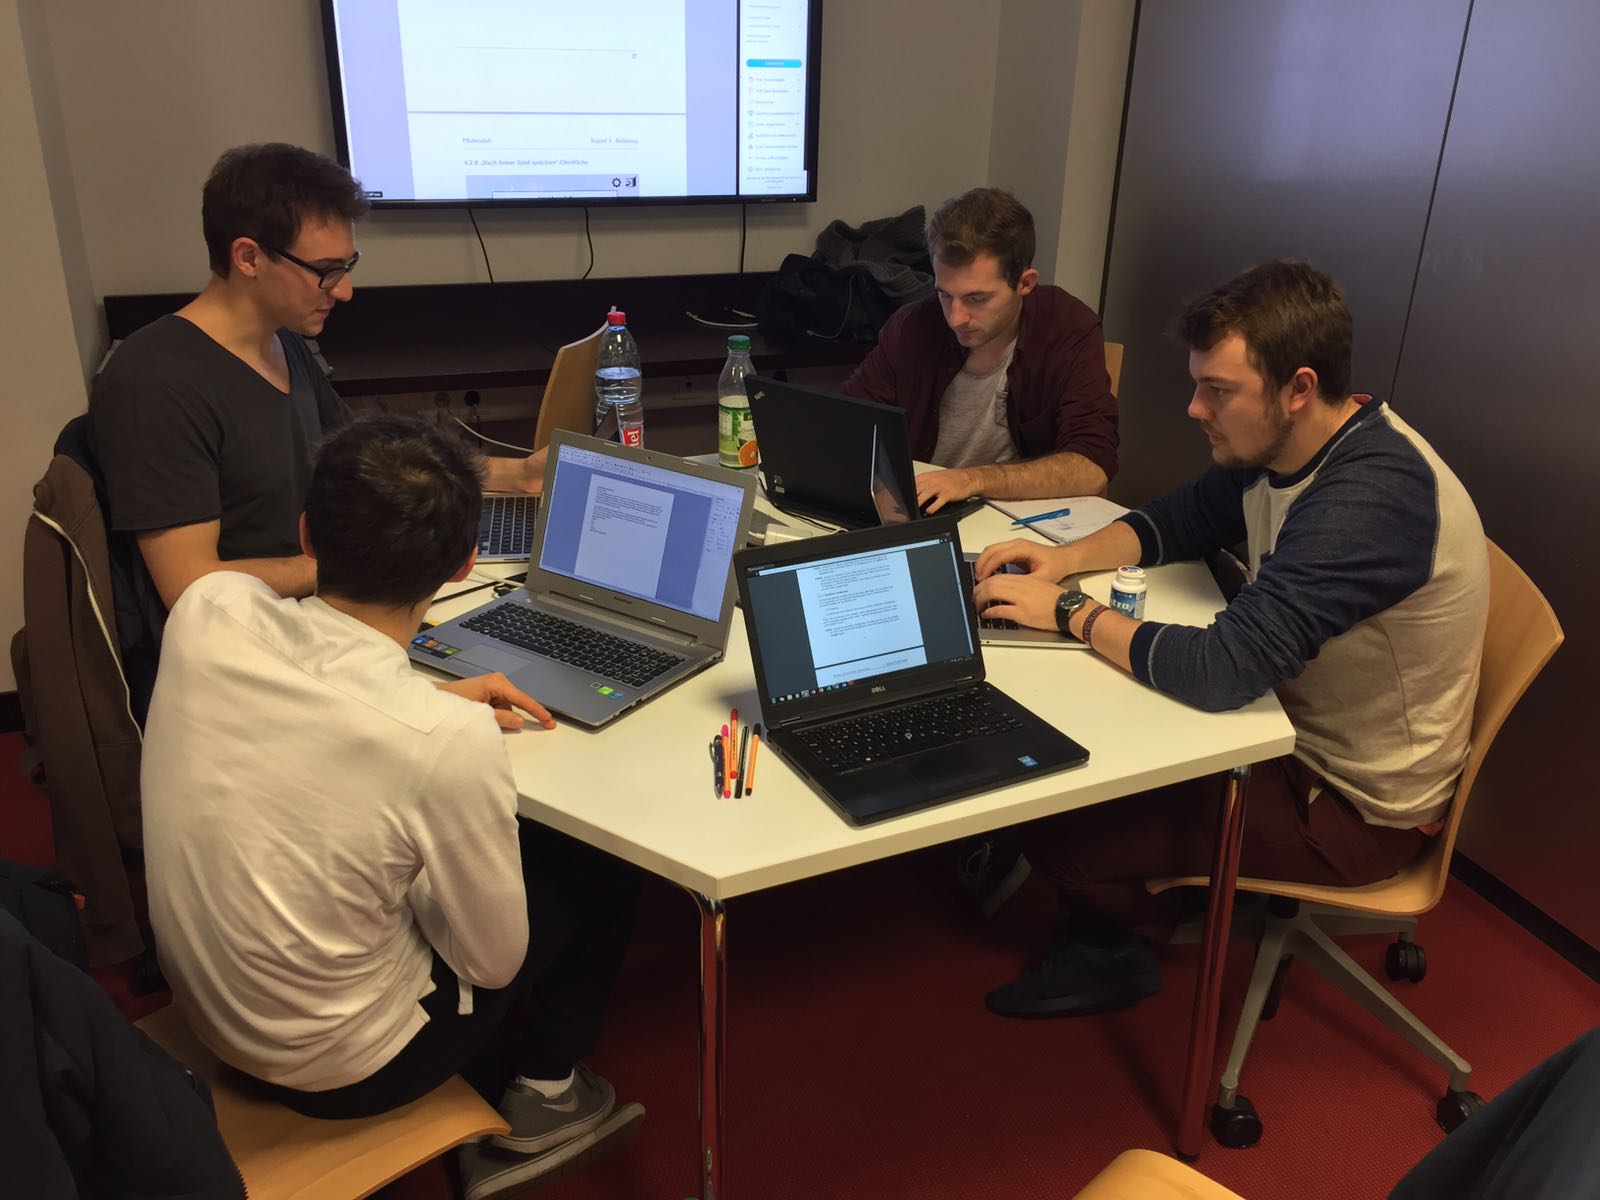
\includegraphics[scale=0.16]{resources/Gruppenarbeit} 
		\end{center}
	\end{figure}	 
\end{frame}

\section{Quellen}
\begin{frame}{Quellen}
	\begin{itemize}
		\item \url{https://www.planetdeadly.com/wp-content/uploads/massive-nuclear-explosion.jpg}
		\item \url{http://www.unternehmer-portal.net/wp-content/uploads/rotes-kreuz-fehler-200x200.png}
		\item \url{http://www.instructables.com/id/Traditional-Portrait-Painting-Step-by-Step/?ALLSTEPS}
		\item \url{http://www.alifechangingjourney.com/wp-content/uploads/2013/01/too-many-thoughts.jpg}
		\item \url{https://de.wikipedia.org/wiki/Mona_Lisa}
	\end{itemize}	
\end{frame}

\end{document}
